%TODO: obviously rewrite this
In this section I will describe the stack used for this thesis and the experiments done to achieve our results: I will start by reviewing the database (Par. \ref{rldb}), the configuration and parameters, the experiments results, and finally the conclusion.

\section{Building Blocks}
To realize this work we used the following tools and libraries:
\begin{itemize}
	\item OpenFace: the library to train the models for face detection, landmark detection, feature extraction and action unit recognition.
	\item R + R-Studio: the environment where I implemented the code, with some important libraries, such as:
	\begin{itemize}
		\item e1071: library for SVM classification.
		\item Tidyverse: General library for %todo
		\item Random Forest: library to perform Random Forest and calculate variable importance.
		\item Corrplot: library for calculating and visualizing correlations.
	\end{itemize}
\end{itemize}

\clearpage

%TODO: SHORT review (table pherhaps) of face db, maybe not in this section
\section{Real Life Trial Database} \label{rldb}
This section is about the database we used to perform our experiments: it comes from the work done for the paper "Deception Detection using Real-life Trial Data" \cite{Perez-Rosas:2015:DDU:2818346.2820758}.

\begin{figure}[H]
	\centering
	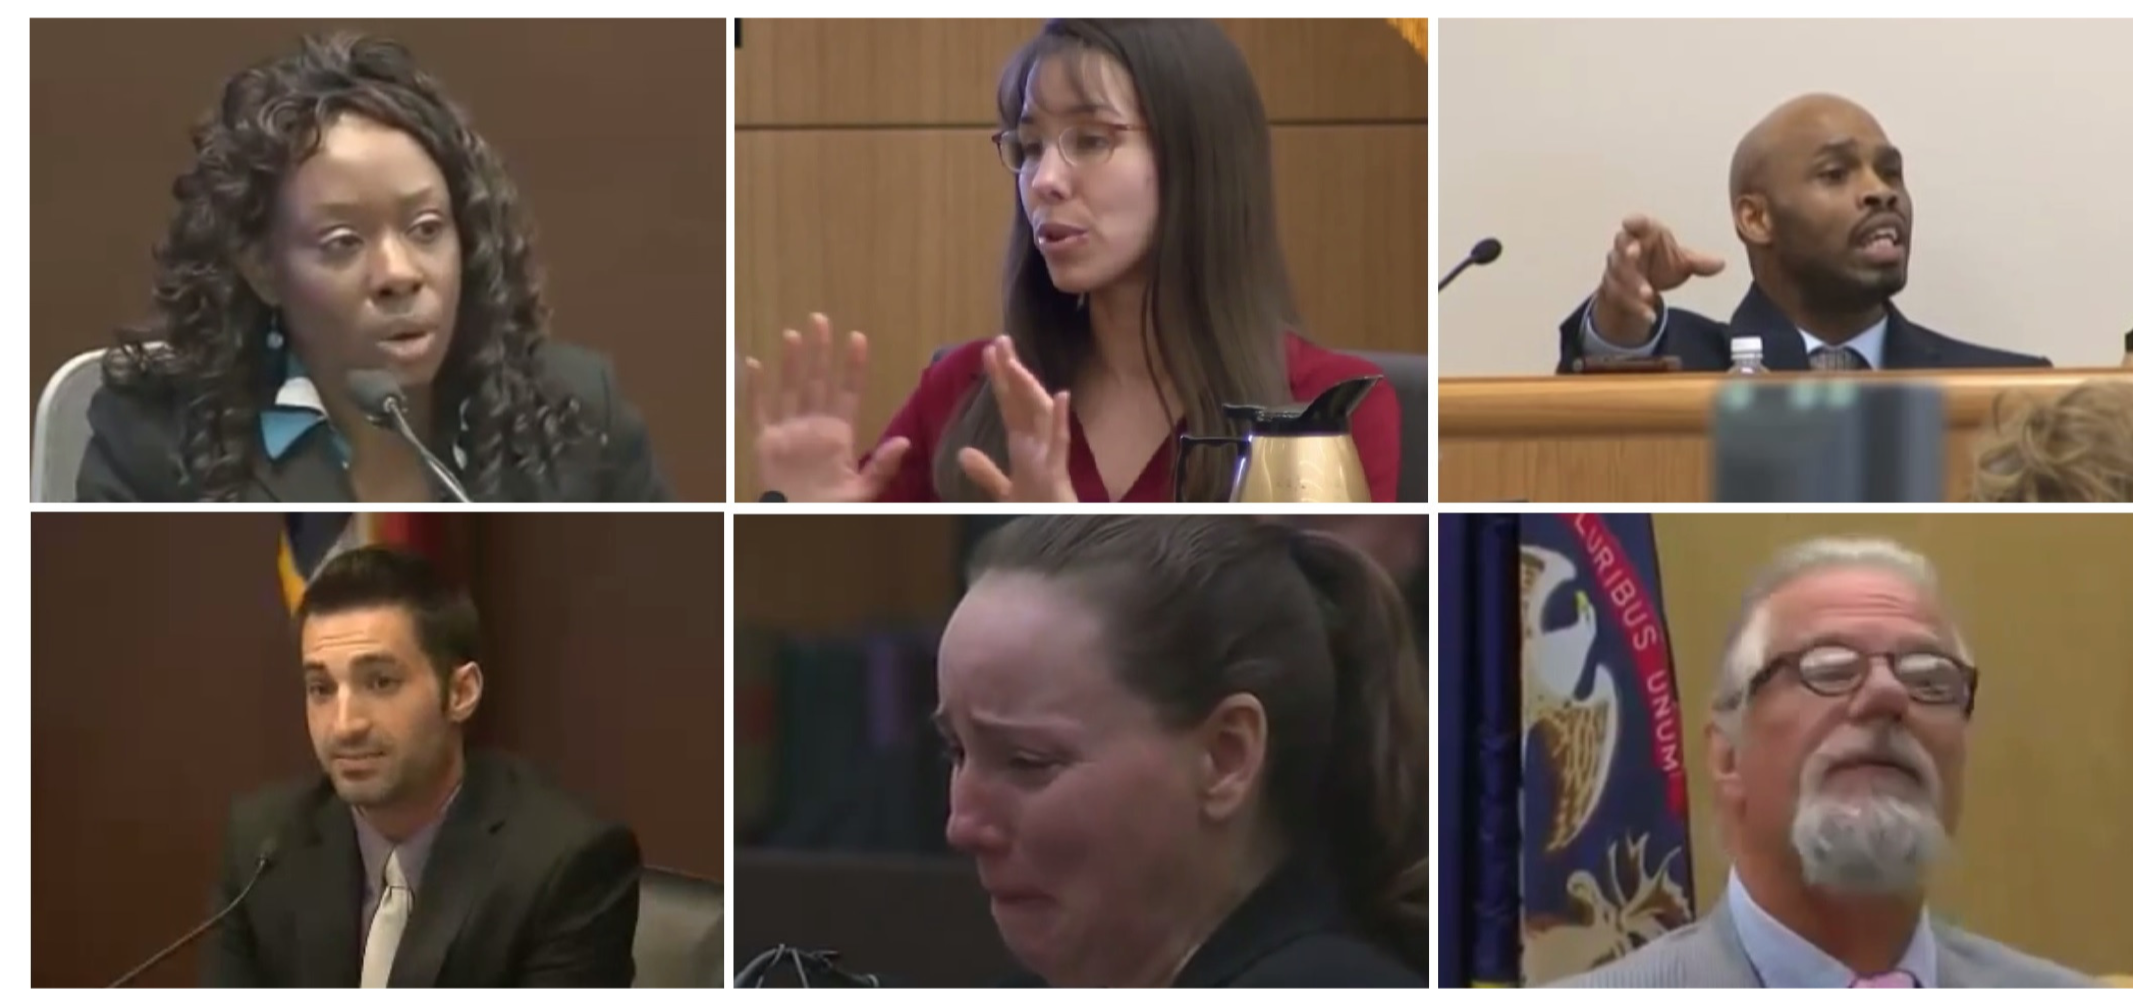
\includegraphics[width=1\textwidth]{trial_images}
	\caption{Examples of images from the dataset videos. \cite{Perez-Rosas:2015:DDU:2818346.2820758}.}
	\label{fig:trial_images}
\end{figure}


The dataset is gathered from real-life trial videos available on YouTube and other public websites. The dataset also contains statements made by exonerees after exoneration, and some statements from defendants during crime-related TV episodes.

The first step to collecting the dataset was to identify public multimedia sources where the recordings of the trials were available, and deceptive and truthful behavior could be observed and verified.\\
The videos are of trial recordings where the defendant or witness in the video can be clearly identified, the face is visible enough during most of the clip duration, and the visual quality should be good enough to accurately see the facial expressions (Fig. \ref{fig:trial_images}).\\
There are three outcomes for the trials that were considered to label the videos as deceptive or truthful: guilty, non-guilty, and exoneration. \\
For the guilty verdicts the deceptive clips are taken from the defendant in the trial, while the truthful clips are gathered from the witnesses. There are also instances where the deceptive videos are of suspects denying a committed crime, and truthful ones are from the same person answering questions that where verified by the police as truthful.

In regards to the witnesses, if the testimony is verified by a police officer they are labeled as true. \\ Testimonies that help the guilty party are labeled as false. Exoneration (reversal of the sentence) testimonies are regarded as truthful.

The original dataset consists of 121 videos, 61 of which are deceptive and 60 truthful. \\
The average length of the videos is 28.0 seconds. The average video length for deceptive videos is 27.7 seconds, while the one for truthful videos is 28.3 seconds. \\
The data consists of 58 total subject, 22 females and 36 males, with ages between 16 and 60 years.

%TODO: modification made by me to the DB 
%TODO: rewrite tentative atm

We modified this database to reduce the amount of videos where the face was hard to see, that had multiple subjects, or where the subjects were not visible while speaking.
Also we performed a division of subjects "by hand" to train the classifiers in a way that it wouldn't "remember" the person, since we have many videos with the same subject. In fact, the same person never appears both in the training and in the test set.

\clearpage

\section{Random Forest}

\section{GLM}

\section{LDA}

\section{QDA}

\section{SVM}

\section{Correlations} ?